%%%%%%%%%%%%%%%%%%%%%%%%%%%%%%%%%%%%%%%%%
% fphw Assignment
% LaTeX Template
% Version 1.0 (27/04/2019)
%
% This template originates from:
% https://www.LaTeXTemplates.com
%
% Authors:
% Class by Felipe Portales-Oliva (f.portales.oliva@gmail.com) with template 
% content and modifications by Vel (vel@LaTeXTemplates.com)
%
% Template (this file) License:
% CC BY-NC-SA 3.0 (http://creativecommons.org/licenses/by-nc-sa/3.0/)
%
%%%%%%%%%%%%%%%%%%%%%%%%%%%%%%%%%%%%%%%%%

%----------------------------------------------------------------------------------------
%	PACKAGES AND OTHER DOCUMENT CONFIGURATIONS
%----------------------------------------------------------------------------------------

\documentclass[
	12pt, % Default font size, values between 10pt-12pt are allowed
	%letterpaper, % Uncomment for US letter paper size
	%spanish, % Uncomment for Spanish
]{fphw}

% Template-specific packages
\usepackage[utf8]{inputenc} % Required for inputting international characters
\usepackage[T1]{fontenc} % Output font encoding for international characters
\usepackage{mathpazo} % Use the Palatino font
\usepackage[dvipsnames]{xcolor}
\usepackage{graphicx} % Required for including images
\usepackage{amsmath}
\usepackage{booktabs} % Required for better horizontal rules in tables
\usepackage{listings} % Required for insertion of code
\usepackage{enumerate} % To modify the enumerate environment
\usepackage{ragged2e}
\usepackage{cancel}
\usepackage{MnSymbol,bbding,pifont}
\usepackage{everyhook}
\usepackage{lscape}
\usepackage{array}
\usepackage{float,graphicx}
\newcommand{\randomcolor}{%
  \definecolor{randomcolor}{RGB}
   {
    \pdfuniformdeviate 256,
    \pdfuniformdeviate 256,
    \pdfuniformdeviate 256
   }%
  \color{randomcolor}%
}

%----------------------------------------------------------------------------------------
%	ASSIGNMENT INFORMATION
%----------------------------------------------------------------------------------------

\title{Assignment \#2} % Assignment title

\author{Luis Alberto Ballado Aradias} % Student name

\date{\today} % Due date

\institute{Centro de Investigación y de Estudios Avanzados del IPN \\ Unidad Tamaulipas} % Institute or school name

\class{Introducción al Análisis de Fourier (Sep - Dec 2022)} % Course or class name

\professor{Dr. Wilfrido Gómez-Flores} % Professor or teacher in charge of the assignment

%----------------------------------------------------------------------------------------


\begin{document}

\maketitle % Output the assignment title, created automatically using the information in the custom commands above

%----------------------------------------------------------------------------------------
%	ASSIGNMENT CONTENT
%----------------------------------------------------------------------------------------

{\color{teal}
  \dotfill
  Función 1
\dotfill}

\begin{minipage}{0.3\textwidth}
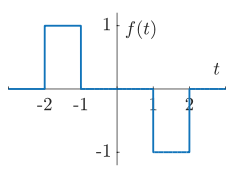
\includegraphics[scale=0.5]{images/func_1.png}
\end{minipage}
\begin{minipage}{0.6\textwidth}\raggedleft
\[f(t) =\left\{ \begin{array}{lr}+1, & -2 < t < -1 \\-1, & 1 < t < 2\\0, & otro\hspace{0.1cm} caso \end{array}\right.\]
\end{minipage}
\noindent

{\color{teal}
  \dotfill
  Transformada de Fourier
\dotfill}
\[\int_{-\infty}^{\infty} f(t) \,e^{-jwt} \,dt \]
\dotfill

\[\int_{-2}^{-1} 1*e^{-jwt} dt + \cancel{\int_{-1}^{1} 0*e^{-jwt} dt} + \int_{1}^{2} -1*e^{-jwt} dt =\int_{-2}^{-1} e^{-jwt} dt - \int_{1}^{2} e^{-jwt} dt \]
Recordando la integral de una exponencial:
\[\int e^{u} du = e^{u} + C \Rightarrow  \frac{-e^{-jwt}}{jw} \Big|_{-2}^{-1} + \frac{-e^{-jwt}}{jw} \Big|_{1}^{2} \]
\[ = \left[\frac{e^{jw}(e^{jw}-1)-e^{-2jw}(e^{jw}-1)}{jw}\right] = \left[\frac{e^{2jw}-e^{jw}-e^{-jw}+e^{-2jw}}{jw}\right]\]
\[ = \left[\frac{e^{2jw}+e^{-2jw}}{jw} - \frac{e^{jw}+e^{-jw}}{jw}\right]*\frac{2}{2} = \frac{2}{w} * \left[\left(\frac{e^{2jw}+e^{-2jw}}{2j}\right) - \left(\frac{e^{jw}+e^{-jw}}{2j}\right)\right]\]

Aplicando identidad:
\[ \frac{2}{w} * \left[\left(\frac{e^{2jw}+e^{-2jw}}{2j}\right) - \left(\frac{e^{jw}+e^{-jw}}{2j}\right)\right] \Rightarrow cos(\theta)=\frac{e^{i\theta}+e^{-i\theta}}{2j} \] 
\begin{center}
\fbox{\begin{minipage}{15em}
\[ \frac{2}{w}*(cos(2w)-cos(w))\]
\end{minipage}}
\end{center}

\newpage
{\color{teal}
\dotfill
Función 1
\dotfill}
\begin{figure}[H]
  \centering
  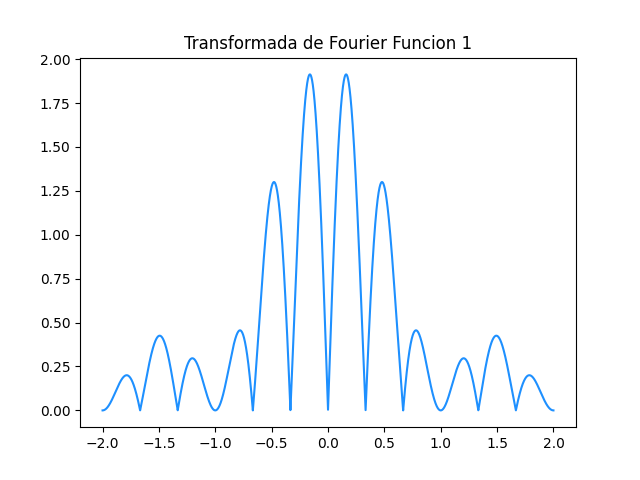
\includegraphics[scale=0.8]{images/trans_fourier_1.png}
\end{figure}

\newpage

{\color{teal}
  \dotfill
  Función 2
\dotfill}

\begin{minipage}{0.3\textwidth}
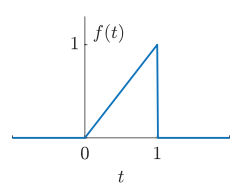
\includegraphics[scale=0.5]{images/func_2.png}
\end{minipage}
\begin{minipage}{0.6\textwidth}\raggedleft
\[f(t) =\left\{ \begin{array}{lr}t, & 0 < t < 1 \\0, & otro\hspace{0.1cm} caso \end{array}\right.\]
\end{minipage}
\noindent

{\color{teal}
  \dotfill
  Transformada de Fourier
\dotfill}
\[\int_{-\infty}^{\infty} f(t) \,e^{-jwt} \,dt \]
\dotfill

\[\int_{0}^{1} t*e^{-jwt} dt \]
\center{Resolviendo la integral por partes}\\
sea $u=t$; $du=dt$;\\
$dv=e^{-jwt}dt$; \\$v=\frac{-e^{-jwt}}{jw}$
\[=\left(\frac{-t*e^{-jwt}}{jw}\right)\Big|_{0}^{1}+\frac{1}{jw}\int_{0}^{1}{e^{-jwt}dt}\]
\[\frac{-1*e^{-jw}}{jw}+\frac{1}{jw}\int_{0}^{1}{e^{-jwt}dt}=\frac{-e^{-jw}}{jw}+\frac{1}{jw}\left(\frac{-e^{-jw}+1}{jw}\right)\]
\[\frac{-e^{-jw}}{jw}-\left(\frac{e^{-jw}-1}{(jw)^{2}}\right)\]
\[ = \left[\frac{-e^{-jw}*jw-e^{-jw}+1}{(jw)^2}\right]\]
\center{Factorizando}
\begin{center}
\fbox{\begin{minipage}{15em}
\[ \frac{e^{-jw}(-jw+e^{jw}-1)}{(jw)^2}\]
\end{minipage}}
\end{center}

\newpage
{\color{teal}
\dotfill
Función 2
\dotfill}
\begin{figure}[H]
  \centering
  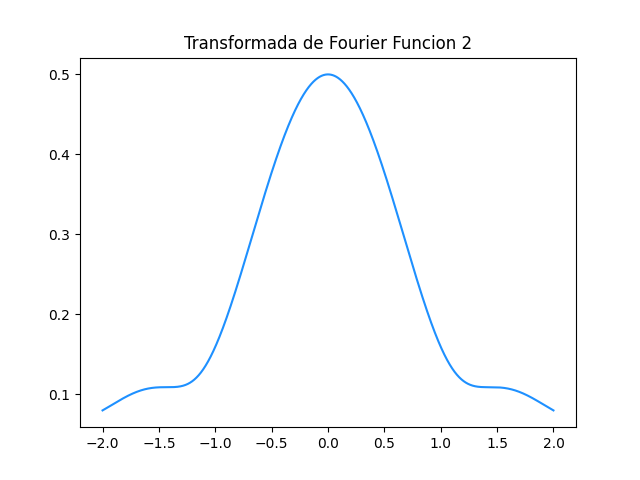
\includegraphics[scale=0.8]{images/trans_fourier_2.png}
\end{figure}

\newpage

{\color{teal}
  \dotfill
  Función 3
\dotfill}

\begin{minipage}{0.3\textwidth}
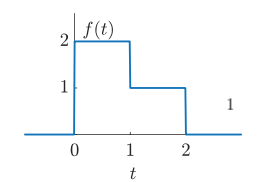
\includegraphics[scale=0.5]{images/func_3.png}
\end{minipage}
\begin{minipage}{0.6\textwidth}\raggedleft
\[f(t) =\left\{ \begin{array}{lr}2, & 0 < t < 1 \\1, & 1 < t < 2 \\0, & otro\hspace{0.1cm} caso \end{array}\right.\]
\end{minipage}
\noindent

{\color{teal}
  \dotfill
  Transformada de Fourier
\dotfill}
\[\int_{-\infty}^{\infty} f(t) \,e^{-jwt} \,dt \]
\dotfill

\[\int_{0}^{1} 2*e^{-jwt} dt + \int_{1}^{2} 1*e^{-jwt} dt + 0 = 2\int_{0}^{1} e^{-jwt} dt + \int_{1}^{2} e^{-jwt} dt + 0 \]

\[2\left(\frac{-e^{-jwt}}{jw}\right) \Big|_{0}^{1} + \frac{-e^{-jwt}}{jw} \Big|_{1}^{2} \]
\[=2\left( \frac{1-e^{-jw}}{jw}\right) +\frac{e^{-2jw}*(e^{jw}-1)}{jw} \]
\[=\frac{2-2*e^{-jw}}{jw} + \frac{e^{-jw}-e^{-2jw}}{jw} = \frac{2-e^{-jw}-e^{-2jw}}{jw} \]
\begin{center}
\fbox{\begin{minipage}{15em}
\[ \frac{2-e^{-jw}(1+e^{-jw})}{jw}\]
\end{minipage}}
\end{center}

{\color{teal}
\dotfill
Función 3
\dotfill}
\begin{figure}[H]
  \centering
  
\includegraphics[scale=0.8]{images/trans_fourier_3.png}
\end{figure}

\newpage
{\color{teal}
\dotfill
Código python
\dotfill}

Con uso de las librerias
\begin{verbatim}
import numpy as np
import math
import matplotlib.pyplot as plt

_x_ = np.linspace(-2,2,10000)
f = []

#iterar para los valores de t
for i in _x_:
    w = 2*np.pi*i
    #f.append(abs((2/w)*(np.cos(2*w)-np.cos(w)))) #Funcion1
    #f.append(abs((np.exp(-1j*w)*(-1j*w+np.exp(1j*w)-1))/((1j*w)*(1j*w)))) #Funcion2
    f.append(abs((2-np.exp(-1j*w)-np.exp(-2j*w))/(1j*w))) #Funcion3
    
plt.plot(_x_,f,color="dodgerblue")
plt.title("Transformada de Fourier Funcion 3")
plt.savefig("trans_fourier_3.png")

\end{verbatim}


%----------------------------------------------------------------------------------------

\end{document}
